\documentclass[12pt,fleqn]{article}\usepackage{../../common}
\begin{document}
Dalga Denklemleri Hesabi

Önce ip üzerinde titreşimlerin hareketi sonucu olan dalga denklemini
türetelim. Bu türetimin bir şeklini [1]'de görmüştük, şimdi [2,3,4] bazlı olarak
tekrar görelim.

Bir ipte dalga onun salınımı ile oluşacak, ve bu salınım sırasında bir anda, tek
bir fotoğraf karesinde görüntü alt soldaki gibi olabilir, 

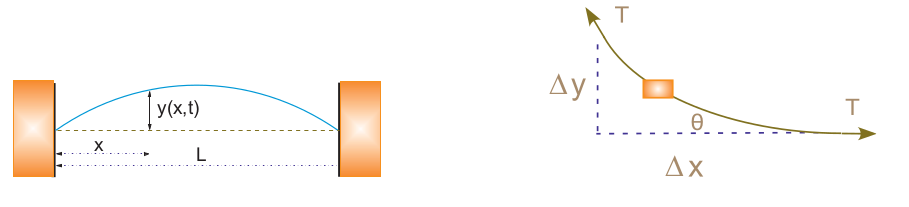
\includegraphics[width=30em]{compscieng_app17wave_01.png}

İp iki tarafından hareket etmeyen yerlere bağlanmış (duvar mesela) uzunluk $L$,
ip materyelinin yoğunluğu $\rho$, ki bu tüm ipin kütlesi bölü uzunluğu olarak ta
görülebilir, bu örnekte sabit, ipin gerginliği kuvvet olarak $T$, bu da sabit,
ve yerçekimi kuvvetine göre çok daha fazla böylece yerçekim ivmelenmesi $g$'yi
yok sayabiliyoruz. Sürtünme yok. Tek boyutta bakıyoruz, $y(x,t)$ ipin bir $x$
noktasındaki dikey yer değişimini gösteriyor.

Denklemi ortaya çıkartmak için aslında Newton'un $F=ma$'sından daha fazlasına
ihtiyacımız yok. Üst sağdaki resimde gösterildiği gibi tek bir sonsuç ufak
bölgeye odaklanırsak, ya da alt resimde olduğu gibi,

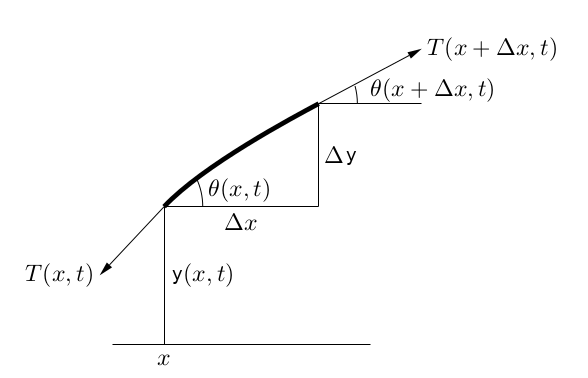
\includegraphics[width=20em]{compscieng_app17wave_02.png}

$F$ için gereken net kuvveti ipin iki yanyana noktası arasındaki gerginliğin
dikey bileşenlerinin farkı olarak görebiliriz, yani $T(x+\Delta x,t)$ ve
$T(x,t)$ kuvvetlerinin dikey bileşen farkı. İki noktadaki acılar da
$\theta(x,t)$ ile gösteriliyor, $x+\Delta x$'teki acı $\theta(x+\Delta x)$. Bu
dikey bileşenlerin farkını, ya da tüm $y$ kuvvetlerinin toplanını o zaman 

$$
\sum F_y = T(x+\Delta x,t) \sin\theta(x+\Delta x,t) - T(x,t) \sin\theta(x,t)
$$

ile hesaplayabiliriz. Modeldeki faraziyeler isiginda biliyoruz ki $y/L$ cok
kucuk, o zaman $\theta$ cok kucuk. Demek ki sinus ifadelerini
basitlestirebiliriz, [5]'ten biliyoruz ki

$$
\sin\theta \approx \tan\theta = \partial y / \partial x
$$

Demek ki

$$
\sum F_y =
T \frac{\partial y}{\partial x} \bigg\vert_{x+\Delta x} -
T \frac{\partial y}{\partial x} \bigg\vert_{x}
$$

Son geldigimiz noktada birinci turevler uzerinden bir $x$ farkliligi goruyoruz,
bu da bize yaklasik olarak ikinci turevi vermez mi? Evet! 

$$
\sum F_y \approx T \frac{\partial^2 y}{\partial x^2}
$$







Kaynaklar

[1] Bayramlı, {\em PDE, Dalga Denklemini Türetmek}

[2] Landau, {\em Landau Computational Physics Course, Video Lectures},
    \url{https://www.youtube.com/playlist?list=PLnWQ_pnPVzmJnp794rQXIcwJIjwy7Nb2U}

[3] Landau, {\em Computational Physics}

[4] Feldman, {\em Math 256, Differential Equations, Lecture Notes}
    \url{http://www.math.ubc.ca/~feldman/m256/}

[5] Bayramli, {\em Normal Diferansiyel Denklemler Ders Notlari, Ekler, Trigonometri}
    
\end{document}
















